\documentclass{emulateapj}

\usepackage{epsfig}
\usepackage{amsmath}
\usepackage{rotating}
\usepackage{natbib}
%\usepackage{lscape}
\usepackage{enumerate}
\usepackage{multirow}
\usepackage{array}
\usepackage{appendix}
\usepackage{comment}
\usepackage{color}

\bibliographystyle{apj}

\def\memoYF#1{\color{red}$[${\bf #1}$]$ \color{black}}

\def\memoDS#1{\color{blue}$[${\bf #1}$]$ \color{black}}

\def\plotonesc#1{\centering \leavevmode
\includegraphics[clip=, width=1.70\columnwidth]{#1}}
\def\plotoneh#1{\centering \leavevmode
\includegraphics[clip=, width=.95\columnwidth]{#1}}
\def\plotone#1{\centering \leavevmode
\includegraphics[clip=, width=.85\columnwidth]{#1}}
\def\plotoneShrinkSmall#1{\centering \leavevmode
\includegraphics[clip=, width=.49\columnwidth]{#1}}
\def\plotoneShrinkMed#1{\centering \leavevmode
\includegraphics[clip=, width=.55\columnwidth]{#1}}
\def\plotoneShrinkBig#1{\centering \leavevmode
\includegraphics[clip=, width=.65\columnwidth]{#1}}
\def\plottwo#1#2{\centering \leavevmode
\includegraphics[width=.45\columnwidth]{#1} \hfil
\includegraphics[width=.45\columnwidth]{#2}}
\def\plottwob#1#2{\centering \leavevmode
\includegraphics[width=.49\columnwidth]{#1} \hfil
\includegraphics[width=.49\columnwidth]{#2}}
\def\plottwor#1#2{\centering \leavevmode
\includegraphics[width=.55\columnwidth,angle=90]{#1} \hfil
\includegraphics[width=.55\columnwidth,angle=90]{#2}}
\def\plotthree#1#2#3{\centering \leavevmode
\includegraphics[width=.3\columnwidth]{#1} \hfil
\includegraphics[width=.3\columnwidth]{#2} \hfil
\includegraphics[width=.3\columnwidth]{#3}}

\newcommand{\cN}[1]{\mathcal{N}}
\newcommand{\pn}[1]{\mbox{$(#1)$}}
\newcommand{\spa}{\mbox{ }}
\def\gsim{\;\rlap{\lower 2.5pt
 \hbox{$\sim$}}\raise 1.5pt\hbox{$>$}\;}
\def\lsim{\;\rlap{\lower 2.5pt
   \hbox{$\sim$}}\raise 1.5pt\hbox{$<$}\;}

% set formatting properties
\setlength{\textwidth}{6.5in}
\setlength{\textheight}{8.8in}
\setlength{\hoffset}{0.0in}
\setlength{\voffset}{-0.4in}
%\setlength{\voffset}{0.3in}
\parindent 0.2in
\parskip 0.1in



%%%%%%%%%%%%%%%%%%%%%%%%%%%%%%%%%%%%%%%%%%%%%%%%%
% THE DOCUMENT BEGINS HERE                      %
%%%%%%%%%%%%%%%%%%%%%%%%%%%%%%%%%%%%%%%%%%%%%%%%%

%\slugcomment{Submitted to ApJ, 20 October 2011}

\begin{document}


%%% Begin front material
%\twocolumn[%%% Begin front material

\title{Red-Giant Hot Jupiters: Brilliant Radio Emitter?}


\author{
%
Yuka Fujii\altaffilmark{0} \\
%
David S. Spiegel\altaffilmark{1, 2} \\
%
{\bf and some order:} \\
%
Jason Nordhaus\altaffilmark{3} \\
%
Nikku Madhusudhan\altaffilmark{4} \\
%
Mehrdad Mirbabayi\altaffilmark{1} \\
%
Aaron Parsons\altaffilmark{5} \\
%
Tony Mroczkowski\altaffilmark{6} \\
%
Neil Zimmerman\altaffilmark{7}
}

\affil{$^0$Earth-Life Science Institute, Tokyo Institute of Technology, 
  Tokyo, JAPAN, 152-8550}
  
\affil{$^1$Astrophysics Department, Institute for Advanced Study,
  Princeton, NJ 08540}

\affil{$^2$Research \& Development, Project Florida Labs,
  New York, NY  10001}

\affil{$^2$Department of Mathematics, Rochester Institute of Technology}

\affil{$^3$Astronomy Department, University of Cambridge, UK}

\affil{$^4$Astronomy Department, UC Berkeley}

\affil{$^5$Naval Research Laboratory}

\affil{$^6$Department of Mechanical and Aerospace Engineering, Princeton University, Princeton, NJ 08544}


\vspace{0.5\baselineskip}

\email{
dave@ias.edu
}


\begin{abstract}
  Red-giant hot Jupiters are jovian planets orbiting red-giant-branch
  or asymptotic-giant-branch (AGB) stars.  Post-main-sequence stars
  lose mass at much higher rates than main-sequence stars.  A jovian
  planet passing through the dense winds of its AGB host can capture
  stellar wind in its magnetosphere.  The cyclotron frequency of
  electrons from the stellar wind accreting onto the planet scales as
  100~MHz~$(B/30 {\rm~Gauss})$.  Such a planet might generate a radio
  luminosity that would be visible from kiloparsec distances.
\end{abstract}


\keywords{planets and satellites: Jupiter --- Sun: evolution ---
  planetary systems --- radiative transfer --- stars: evolution ---
  stars: AGB and post-AGB}
%]%%% End front material

%%%%%%%%%%%%%%%%%%%%%%%%%%%%%%%%%%%%%%%%%%%%%%%%%%%%%%%%%%%%%%%%%%%
\section{Introduction}
\label{sec:intro}
%%%%%%%%%%%%%%%%%%%%%%%%%%%%%%%%%%%%%%%%%%%%%%%%%%%%%%%%%%%%%%%%%%%



Planets with strong magnetic fields may generate radio or X-ray emission when interacting with energetic charged particles. 
It has been known that Jupiter emits radio emission from the radiation belt and auroral region due to the acceleration of the plasmas. \memoYF{?}. Potentially, large exoplanets can also emit radio waves through the similar mechanisms, depending on their intrinsic magnetic fields and the density of surrounding plasmas, e.g. stellar wind particles and particles from Io-like moons. 
Radio emissions from exoplanets have been estimated taking account of several possible processes, based on the empirical scaling of the radio intensity with the solar wind flux \citep{zarka2001,griebmeier2007,noyola2013}. 
Although the search for these radio signatures are being conducted, there is no clear detection claimed so far, while some indications were obtained \memoYF{?} \citep{lecavelier_et_al2013}. 
%In general, there are four proposed models for a planet to emit radio wave \citep{griebmeier2007}: 1) the magnetic energy model, 2) kinetic energy model, 3) CME model, and 4) the unipolar interaction model. 
%The search for these radio emissions from extrasolar Jovian planets has been performed. 


%It has been predicted that
% fix
When stars less than $\sim$8~$M_\sun$ evolve off the main sequence,
they go through stages on the red-giant branch (RGB) and the
asymptotic-giant branch (AGB) where their radii and luminosities increase by orders of magnitude. 
Jovian planets in orbit around such stars can be transiently heated to hot-Jupiter temperatures ($\sim$1000~K or more) at distances out to tens of AU, depending on the star's mass \citet{spiegel+madhusudhan2012}. 
At the same time, they are subject to massive stellar wind, because the mass-loss rate of such evolved stars are significantly higher than the main-sequence counterparts, typically $\sim  10^{-8} M_{\odot }$/yr \citep{judge1991}. \memoYF{How these values are observationally obtained?} \memoYF{Dave mentioned $\sim  10^{-5} M_{\odot }$/yr, where does this come from?} through massive (but slow) stellar wind \citep{suzuki2008} \memoYF{cite more papers?}. 
On the assumption that the radio emission is correlated with the stellar wind, planetary companions around evolved stars could generate bright radio emission. 

In this paper we propose the potential to detect planetary companions around evolved stars through the brightness of their radio emission. 
The search for such emission could tell us the population of companions around evolved stars, including those were originally A or O stars. 

In \S2, we discuss the assumption we make in this paper. 
\S3, we provide the estimates. 
\S4, we examine the possible obstacles to detect radio emission from the companion, taking account of the intrinsic radio emission of the evolved stars...
% based on the number of targets in the observable volumes


%Red giants lose their masses at a high rate, typically $\sim  10^{-5} M_{\odot }/yr $ through massive stellar wind. These stellar wind particle can 


%Roughly 20\% of the more than 700 \memoYF{check!} currently known exoplanets around main-sequence stars \footnote{See online catalogs such as http://www.openexoplanetcatalogue.com/ \citep{rein2012}, http://exoplanet.eu \citep{schneider_et_al2011}, or http://exoplanets.org \citep{wright_et_al2011} for up-to-date lists.} have masses greater than half of Jupiter's, orbital radii greater than 1~AU, and will become hot Jupiters (i.e., for the present purposes, this means they will receive at least as much irradiation as the currently known hot Jupiters/Neptunes \citep{spiegel+madhusudhan2012}. 


%%%%%%%%%%%%%%%%%%%%%%%%%%%%%%%%%%%%%%%%%%%%%%%%%%%%%%%%%%%%%%%%%%%
\section{Assumptions}
\label{s:assumptions}
%%%%%%%%%%%%%%%%%%%%%%%%%%%%%%%%%%%%%%%%%%%%%%%%%%%%%%%%%%%%%%%%%%%

%%%%%%%%%%%%%%%%%%%%%%%%%%%%%%%%%%%%%%%%%%%%%%%%%%%%%%%%%%%%%%%%%%%
\subsection{Mechanisms}
\label{ss:mechanisms}
%%%%%%%%%%%%%%%%%%%%%%%%%%%%%%%%%%%%%%%%%%%%%%%%%%%%%%%%%%%%%%%%%%%


Radio emission intensity of Solar System giant planets are known to be proportional to the kinetic energy or the magnetic energy of the solar wind,  which interacts with planetary magnetic field at the magnetic standoff cross section\memoYF{``radio Bode's law'': cite something}. 

Unfortunately, the detail of the mechanism of energy transport from the energy source into the radio emission. 




According to \citet{griebmeier2007} \memoYF{The following equations are quoted from the paper. Needs to elaborate. }
\begin{enumerate}
\item kinetic energy model
\begin{equation}
P_{\rm inp} \propto n v^3 r_s ^2 \label{eq:Pinp_kin}
\end{equation}
\item magnetic energy model:
\begin{equation}
P_{\rm inp} \propto v B_{\bot }^2 r_s ^2 \label{eq:Pinp_mag}
\end{equation}
\item CME model\\
Not sure about CME for red giants. We don't consider?
\item the unipolar interaction model\\
??
\end{enumerate}
where $n$ and $v$ are density and velocity of stellar wind, respectively,  $ B_{\bot }$ is the interstellar magnetic field perpendicular to the stellar wind flow, and $r_s$ is the radius of magnetic standoff point. 



%%%%%%%%%%%%%%%%%%%%%%%%%%%%%%%%%%%%%%%%%%%%%%%%%%%%%%%%%%%%%%%%%%%
\subsection{Properties for Stellar Wind of RGs}
\label{ss:stellarwind}
%%%%%%%%%%%%%%%%%%%%%%%%%%%%%%%%%%%%%%%%%%%%%%%%%%%%%%%%%%%%%%%%%%%

The mass loss rate of the stellar wind can be estimated from observation \memoYF{How?}.
For the known red giants, the values are typically $\dot M \sim 10^{-8} M_{\odot}$/yr, and can be as high as $10^{-5} M_\odot~{\rm yr^{-1}}$ during AGB phases, significantly greater than the solar mass-loss rate $\sim 10^{-14} M_{\odot}$/yr. 

%\memoDS{Can be as high as $10^{-5} M_\odot~{\rm yr^{-1}}$ during AGB phases.  I'm calling it ``red giant'' but we're really thinking of AGB stars for maximum mass-loss and brightness.}
%>>>>>>> e6e562d36dff6e5bb10b57fdd066ee5edd32b496
\begin{equation}
\frac{\dot M}{\dot M_{\odot}} \sim 10^6
\end{equation}

The stellar wind velocity becomes smaller because of the small escape velocity (due to expanded stellar radius)\footnote{Escape velocity is $\sqrt{2GM/r}$.}. Assuming that the stellar wind scales as the escape velocity, RGs with radius $R=100R_{\odot}$ have 10 times as slow stellar wind as that at the main sequence.
\begin{equation}
\frac{v}{v_{\odot}} \sim 10^{-1}
\end{equation}

The temperature of stellar wind of RGs is expected to be 2 orders of magnitude lower than their main sequence counterparts, mainly because the sound speed of hot corona exceeds the escape speed, i.e., hot corona cannot be confined in the stellar atmosphere \citep{suzuki2008}. 
\begin{equation}
\frac{T}{T_{\odot}} \sim 10^{-2}
\end{equation}

%%%%%%%%%%%%%%%%%%%%%%%%%%%%%%%%%%%%%%%%%%%%%%%%%%%%%%%%%%%%%%%%%%%
\subsection{Properties for Planetary Magnetic Field}
\label{ss:planetarymagnetic}
%%%%%%%%%%%%%%%%%%%%%%%%%%%%%%%%%%%%%%%%%%%%%%%%%%%%%%%%%%%%%%%%%%%

Theoretically, the magnetic moment of gaseous planets are expressed with the following scaling relationship \citep{griebmeier2004}:
%%%%%%%%%% 
\begin{equation}
\mathcal{M} \propto  \omega ^{\alpha } \rho_c ^{\beta } r_c^{\gamma } \sigma ^{\delta }
\end{equation}
%%%%%%%%%%
where $\omega $ is the spin angular velocity, $\rho _c$, $r_c$ and $\sigma $ are the density, the radius, and the conductivity of the ``dynamo region'' where the density is high enough for hydrogen to be metallic, respectively. 
The scaling indexes are estimated to be $\alpha \sim 1/2-1$, $\beta \sim 1/2$, $\gamma \sim 3-4$, and $\sigma \sim -1/2-0$. In this paper, we assume $\alpha =1$, $\beta =1/2$, and $r_c = 7/2$ \citep{sano1993}. \memoYF{validity?}

Unlike usual hot jupiters, RGHJs are not subject to tidal lock, because the gravitational effects of their host star does not change even if the star evolves into red giants. Without no physical insights of the typical spin period, we simply assume that of Jupiter: $\omega = 9.925$ [hr]. 

In order to evaluate $\rho _c $ and $r_c$, we need a model of internal structure of gaseous planets. We simply use the same model as \citet{griebmeier2004}, where the density as a function of radius from the center is described as:
%%%%%%%%%% 
\begin{equation}
\rho (r) = \left( \frac{\pi M_p}{4 R_p^3} \right) \frac{\sin \left( \pi \frac{r}{R_p} \right)}{\left( \pi \frac{r}{R_p} \right)} \label{eq:rho_r}
\end{equation}
%%%%%%%%%%
where
%%%%%%%%%% 
\begin{equation}
R_p (M_p) = \frac{(\alpha M_p)^{1/3}}{1+\left( \frac{M_p}{M_{\rm max}} \right)} \label{eq:Rp}
\end{equation}
%%%%%%%%%%
with $\alpha =6/1 \times 10^{-4}$ \citep{griebmeier2007}. 
We determine the core radius $r_c$ by assuming that the hydrogen becomes metallic when $\rho (r)$ exceeds the critical density $\rho_c=700\,\mbox{kg/m}^3$. The density of the metallic core, $\rho _c$ is obtained by averaging the density in the core. 
We assume that the conductivity $\sigma $ is the same as Jupiter \memoYF{?}. 


%%%%%%%%%%%%%%%%%%%%%%%%%%%%%%%%%%%%%%%%%%%%%%%%%%%%%%%%%%%%%%%%%%%
\section{Estimates of Radio Emission from RGHJ}
\label{s:estimate}
%%%%%%%%%%%%%%%%%%%%%%%%%%%%%%%%%%%%%%%%%%%%%%%%%%%%%%%%%%%%%%%%%%%

%%%%%%%%%%%%%%%%%%%%%%%%%%%%%%%%%%%%%%%%%%%%%%%%%%%%%%%%%%%%%%%%%%%
\subsection{Estimates of frequency}
\label{ss:frequency}

The cyclotron frequency is
\begin{eqnarray}
f_{\rm cyclotron} &=& \frac{eB}{2\pi m_e c} \approx 28 {\rm~MHz} \left( \frac{B}{10 \rm~G} \right) \, ,
\label{eq:cyc} \\
B &=& \frac{\mu_0}{2\pi}\frac{\mathcal{M}}{R_p^3} \\
&\sim & 9.1 \mbox{[G]} \left( \frac{\mathcal{M}}{\mathcal{M}_J} \right) \left( \frac{R_p}{R_{p, J}} \right)^{-3}. 
\end{eqnarray}
%where $\mathcal{M}_J = 1.56 \times 10^{27} \mbox{A m}^2$. 
For magnetic field strengths in the vicinity of $\sim$25-50~Gauss (G),
the cyclotron frequency will be in the range $\sim$75-150~MHz.

Figure \ref{fig:f_cyclotron} shows the cyclotron frequency of the planetary magnetic field. 

%%%%%%%%%%%%%%%%%%%%%%%%%%%%%%%%%%%                                                                                                                                               
\begin{figure}[!h]
\begin{center}
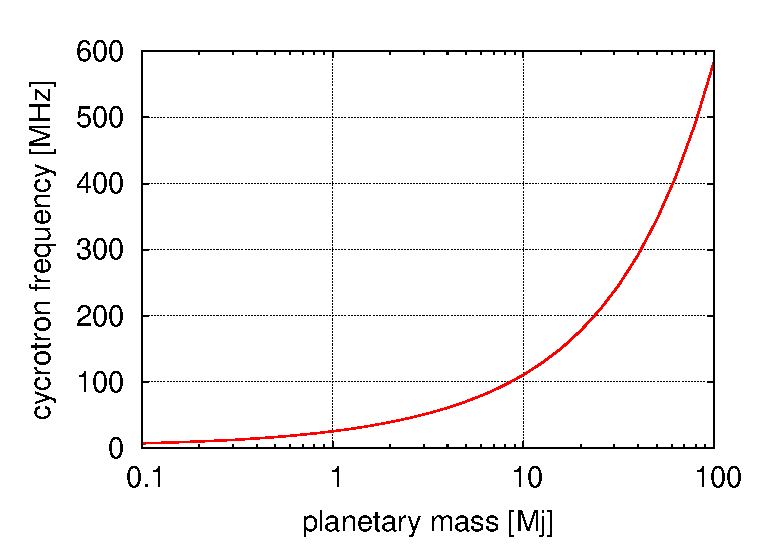
\includegraphics[width=0.7\hsize]{test_fcycrotron.eps}
\end{center}
\caption{Cyclotron frequency. (May be deleted eventually.)}
\label{fig:f_cyclotron}
\end{figure}
%%%%%%%%%%%%%%%%%%%%%%%%%%%%%%%%%%% 


The emission is observable only when the maximum frequency is larger than the plasma frequency of the surrounding stellar wind. 
The plasma frequency is 
\begin{eqnarray}
f_{\rm plasma} &=& \frac{1}{2\pi} \sqrt{\frac{ne^2}{\epsilon _0 m_e}} \\
&\approx & 4\mbox{[MHz]} \left( \frac{\dot M}{10^6 \dot M_{\odot}}\right)^{1/2} \left(\frac{v}{10^{-1} v_{\odot}}  \right)^{-1/2}
\end{eqnarray}

%%%%%%%%%%%%%%%%%%%%%%%%%%%%%%%%%%%                                                                                                                                               
\begin{figure}[!h]
\begin{center}
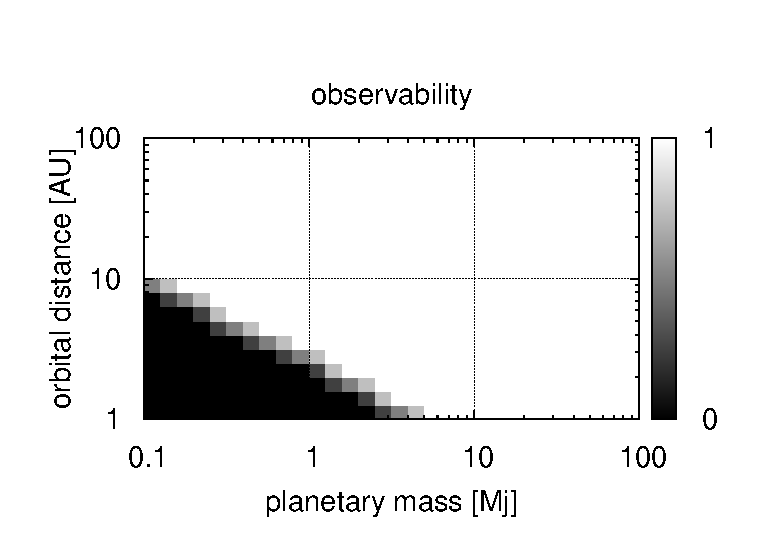
\includegraphics[width=0.9\hsize]{test_observability.eps}
\end{center}
\caption{Where condition $f_{cyclotron}>f_{plasma}$. (May be deleted eventually.)}
\label{fig:f_cyclotron}
\end{figure}
%%%%%%%%%%%%%%%%%%%%%%%%%%%%%%%%%%% 


%%%%%%%%%%%%%%%%%%%%%%%%%%%%%%%%%%%%%%%%%%%%%%%%%%%%%%%%%%%%%%%%%%%
\subsection{Estimates of intensity}
\label{ss:intensity}

$r_s$ is determined by the balance between the magnetic pressure of planetary magnetosphere and kinetic pressure of stellar wind\footnote{Precisely, the magnetic standoff point is described by equation (9) of \citet{griebmeier2007}, which is. 
\begin{equation}
r_s = \left[ \frac{\mu_0 f_0^2 \mathcal{M}}{8\pi^2 (m_p n(d) v(d)^2 + 2 n(d) k_B T)} \right]^{1/6}
\end{equation}
where $\mathcal{M}$ is the planetary magnetic moment and $m_p$ is the proton mass. 
In the following arguments based on Dave's sketch, the second term in the denominator is ignored. This is valid for Solar wind where the first term is larger than the second term by 2 orders of magnitude. \memoYF{check!}}. Thus, 
\begin{equation}
\frac{m_p n v ^2}{2} = \frac{B^2}{2\pi}\left( \frac{r_s}{R_p} \right)^{-6} 
\end{equation}
Therefore,
\begin{eqnarray}
r_s &=& R_p \left( \frac{B^2}{\pi \dot M v (1/4\pi d^2)} \right)^{1/6} = R_p \left( \frac{4 B^2 d^2}{\dot M v } \right)^{1/6} \\
&\approx & 5 R_J \left(\frac{B}{10 \mbox{[G]}}\right)^{1/3} \left(\frac{\dot M}{10^6 \dot M_{\odot}}\right)^{-1/6}\\
&& \;\;\;\;\; \;\;\;\;\; \times \left(\frac{v}{10^{-1} v_{\odot}}\right)^{-1/6}  \left(\frac{d}{5 \mbox{[AU]}}\right)^{1/3} 
\end{eqnarray}

Therefore, the radio emission expected from kinetic energy model (equation (\ref{eq:Pinp_kin})) is 
\begin{eqnarray}
P_{\rm radio} &=& P_{\rm radio, J} \left(\frac{\dot M }{\dot M_{\odot }} \right) \left(\frac{v}{v_{\odot}} \right) ^2 \left(\frac{d}{5 \rm{AU}} \right) ^{-2}  \left(\frac{r_s}{r_{s, {\rm J}}} \right)^2 \\
&=& P_{\rm radio, J} \left(\frac{\dot M }{\dot M_{\odot }} \right)^{\frac{2}{3}} \left(\frac{v}{v_{\odot}} \right) ^{\frac{5}{3}} \left(\frac{d}{5 \rm{AU}} \right) ^{-2} \left(\frac{B}{B_J} \right)^{\frac{2}{3}} \\
&\approx& 200 P_{\rm radio, J} \left(\frac{\dot M }{10^6 \dot M_{\odot }} \right)^{\frac{2}{3}} \left(\frac{v}{10^{-1} v_{\odot}} \right) ^{\frac{5}{3}} \\
&& \;\;\;\;\; \;\;\;\;\; \times \left(\frac{d}{5 \rm{[AU]}} \right) ^{-4/3} \left(\frac{B}{10 \mbox{[G]}} \right)^{\frac{2}{3}} \
\end{eqnarray}


\memoYF{Following arguments are based on \citep{griebmeier2007}. }
Assuming $P_{\rm inp, J} = 2.1\times 10^{11}$ W \citep{griebmeier2007}, observed RGHJ radio emission at distance $l$ is
\begin{eqnarray}
P_{\rm obs} &=& \frac{P_{\rm radio}}{\Omega l^2 f_{\rm cyclotron}} \\
&\approx & 5\times 10^{-6} \mbox{Jy} \left( \frac{P_{\rm radio}}{P_{\rm radio, J}} \right) \left( \frac{l}{10\mbox{[pc]}} \right)^{-2} \left( \frac{B}{10\mbox{[G]}} \right) ^{-1} \\
&\approx & 10^{-3} \mbox{Jy} \left( \frac{P_{\rm radio}}{200 P_{\rm radio, J}} \right) \left( \frac{l}{10\mbox{[pc]}} \right)^{-2} \left( \frac{B}{10\mbox{[G]}} \right) ^{-1}
\end{eqnarray}
where $\Omega $ is the solid angle of emission, which is assumed $\Omega = 1.6$. 


Figure \ref{fig:radio} shows the intensity of radio emission from RGHJs. 
%%%%%%%%%%%%%%%%%%%%%%%%%%%%%%%%%%%                                                                                                                                               
\begin{figure}[!h]
\begin{center}
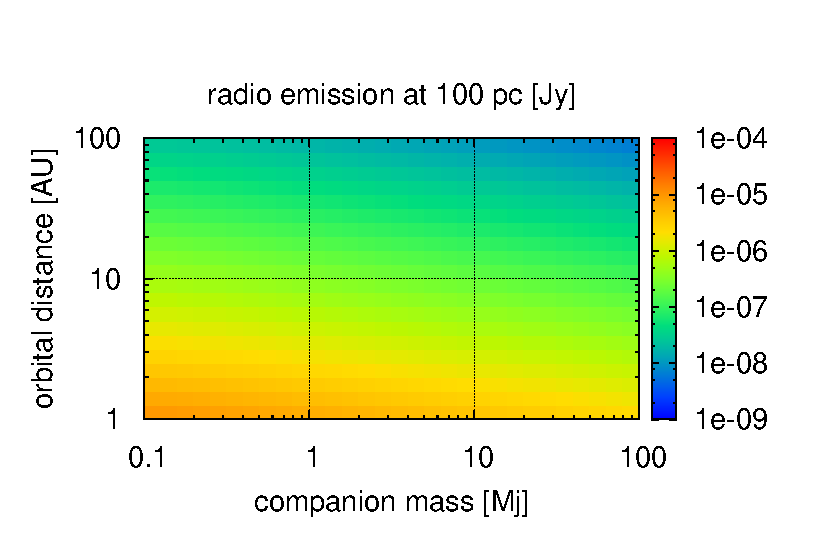
\includegraphics[width=0.9\hsize]{test_radio.eps}
\end{center}
\caption{Intensity of radio emission. }
\label{fig:radio}
\end{figure}
%%%%%%%%%%%%%%%%%%%%%%%%%%%%%%%%%%% 



%%%%%%%%%%%%%%%%%%%%%%%%%%%%%%%%%%%%%%%%%%%%%%%%%%%%%%%%%%%%%%%%%%%
\subsection{Will the electron spiraling and offset the magnetic field? (Mehrdad Mirababayi)}
\label{ss:offset}


%%%%%%%%%%%%%%%%%%%%%%%%%%%%%%%%%%%%%%%%%%%%%%%%%%%%%%%%%%%%%%%%%%%%%%%%
\newpage

%%%%%%%%%%%%%%%%%%%%%%%%%%%%%%%%%%%%%%%%%%%%%%%%%%%%%%%%%%%%%%%%%%%
\section{Discussion on Observability}
\label{s:discussion}
%%%%%%%%%%%%%%%%%%%%%%%%%%%%%%%%%%%%%%%%%%%%%%%%%%%%%%%%%%%%%%%%%%%


%%%%%%%%%%%%%%%%%%%%%%%%%%%%%%%%%%%%%%%%%%%%%%%%%%%%%%%%%%%%%%%%%%%
\subsection{Radio emission from red giants stars}
\label{ss:RGradio}

(Jason)

\citet{gorman2013}

%%%%%%%%%%%%%%%%%%%%%%%%%%%%%%%%%%%%%%%%%%%%%%%%%%%%%%%%%%%%%%%%%%%
\subsection{Expected population of RGHJ in the observable volume}
\label{ss:number}

\newpage


\section{Dave's sketch}

\citep{spiegel2008}

\citep{lecavelier_et_al2013}

\citep{janhunen_et_al2003}

\citep{zarka1992, zarka1998}

\citep{farrell_et_al2004}

\citep{lazio+farrell2007}: likelihood function, tau Boo search

\citep{lecavelier_et_al2009}

\citep{spiegel2012}

\citep{nordhaus+spiegel2013}



\citep{jiang+jin1996}: 12cm radio of Jupiter during Shoemake-Levy-9

\citep{morin2012, morin_et_al2013}

\citep{christensen_et_al2009, christensen2010}

\citep{saar2001}: Inverse rossby number scaling of magnetic field: $B
\sim 60 {\rm~G} \times Ro^{-1.2}$.  Here, he takes $Ro = \tau_c/P_{\rm
  rot}$, where $\tau_c$ is the convective turnover time = ?
\citep{gilliland1986}.  Well, $F \sim \rho v_c^3 \sim \rho
(H/\tau_c)^3$, so $\tau_c \sim H (\rho / F)^{1/3} = H / (\sigma T_{\rm
  eff}^4 / \rho)^{1/3}$.  Alternatively, $\tau_{\rm conv} \sim (M R^2
/ L)^{1/3}$.

On dimensional grounds, the convective turnover time goes as
$\tau_{\rm conv} \sim (M R^2 / L)^{1/3}$.  According to
\citet{burrows_et_al2001}, radius $R$ and luminosity scale with time
as $R \sim R_J$, where $R_J$ is the radius of Jupiter, and
\begin{equation}
\frac{L}{10^{-9} L_\odot} \sim \left( \frac{t}{1 \rm~Gyr} \right)^{-1.3} \left( \frac{M}{1~M_J} \right)^{2.64} \, .
\label{eq:burrowsLum}
\end{equation}
So,
%\begin{eqnarray}
%\nonumber \tau_{\rm conv} & \sim & 3 {\rm~days} \times \left( \frac{M}{M_J} \right)^{1/3} \left( \frac{R}{R_J} \right)^{2/3} \left( \frac{L}{L_\odot} \right)^{-1/3} \\
% & = & 
%\end{eqnarray}
\begin{eqnarray}
\nonumber \tau_c & \sim & 3 {\rm~hrs} \times \frac{\left( \frac{H}{100 \rm~km} \right) \left( \frac{\rho}{10^{-5} \rm~g~cm^{-3}} \right)^{1/3}}{\left( \frac{L}{10^{-9} L_\odot} \right)^{1/3}} \\
 & = & 3 {\rm~hrs} \times \frac{\left( \frac{H}{100 \rm~km} \right) \left( \frac{\rho}{10^{-5} \rm~g~cm^{-3}} \right)^{1/3}}{\left( \frac{M}{1 ~M_J} \right)^{0.88} \left( \frac{t}{1 \rm~Gyr} \right)^{0.43}} \\
\end{eqnarray}
So the Rossby number $Ro = \tau_c/P_{\rm rot}$ is
\begin{eqnarray}
Ro & = & \frac{\tau_c}{P_{\rm rot}} \\
 & = & \left( \frac{P_{\rm rot}}{3 \rm~hrs} \right)^{-1} \times \frac{\left( \frac{H}{100 \rm~km} \right) \left( \frac{\rho}{10^{-5} \rm~g~cm^{-3}} \right)^{1/3}}{\left( \frac{M}{1 ~M_J} \right)^{0.88} \left( \frac{t}{1 \rm~Gyr} \right)^{0.43}}
\end{eqnarray}

\citep{hallinan_et_al2013}

\citep{desch+kaiser1984} radiometric Bode's law

Noting that
\begin{equation}
\dot{M}_* = 4\pi r^2 \rho[r] v \, ,
\label{eq:mdot
}\end{equation}
so $\rho[r] = \dot{M}_*/(4\pi r^2 v)$,
\begin{eqnarray}
\frac{\rho v^2}{2} = \frac{B^2}{8\pi} \sim \frac{B_0^2}{8\pi} \left( \frac{d}{d_0} \right)^{-3} \, ,
\end{eqnarray}
where $B_0$ is the field strength at a distance $d_0$ from the planet.
\begin{eqnarray}
\frac{\rho v^2}{2} & \sim & \frac{B_0^2}{8\pi} \left( \frac{d}{d_0} \right)^{-6} \\
\frac{\dot{M}_* v}{8\pi a^2} & = & \frac{B_0^2}{8\pi} \left( \frac{d}{d_0} \right)^{-6} \\
\frac{\dot{M}_* v}{r^2} & = & B_0^2 \left( \frac{d}{d_0} \right)^{-6} \\
d^6 & = & \frac{d_0^6 B_0^2 r^2}{\dot{M}_* v} \\
d_A & = & d_0 \left( \frac{B_0^2 r^2}{\dot{M}_* v} \right)^{1/6} \\
  & \sim & 4 R_J \left( \frac{d_0}{R_J}\right) \left\{ \frac{\left( \frac{B}{10 \rm~G} \right)^2 \left( \frac{r}{5 \rm~AU} \right)^2}{\left( \frac{\dot{M}_*}{10^{-6} M_\odot/\rm yr} \right) \left( \frac{v}{20 \rm~km/s} \right)} \right\}^{1/6}
\label{eq:Chapman-Ferraro}
\end{eqnarray}
In the above, $d_A$ is the distance from the planet to the Alfven
point, where the magnetic energy density $u_B = B^2 / 8\pi$ equals the
kinetic energy density in the stellar wind $u_w = \rho v^2/2$, and
$B_0$ is the magnetic field strength at distance $d_0$.

The escape speed is
\begin{equation}
v_{\rm esc}^* = \sqrt{\frac{2 G M_*}{R_*}} \, ,
\end{equation}
so if the stellar wind speed is a factor $C$ times the escape speed, then ...

The power incident on the planet within $d_A$ is
\begin{eqnarray}
P_{\rm inc} & = & \frac{\rho v^3}{2} \times \pi d_A^2 \\
\frac{\rho v^2}{2} & \sim & \frac{B_0^2}{8\pi} \left( \frac{d}{d_0} \right)^{-6} \\
d_A^6 & = & d_0^6 \frac{B_0^2}{4\pi \rho v^2} \\
d_A^2 & = & d_0^2 \left( \frac{B_0^2}{4\pi \rho v^2}\right)^{1/3} \\
\pi d_A^2 \frac{\rho v^3}{2} & = & \frac{d_0^2}{2} \left( \frac{\pi^2 \rho^2 v^7 B_0^2}{4} \right)^{1/3} \\
P_{\rm inc} & = & d_0^2 \left( \frac{\pi^2 \rho^2 v^7 B_0^2}{32} \right)^{1/3} 
%\frac{\dot{M}_* v}{8\pi a^2} & = & \frac{B_0^2}{8\pi} \left( \frac{d}{d_0} \right)^{-6} \\
%\frac{\dot{M}_* v}{r^2} & = & B_0^2 \left( \frac{d}{d_0} \right)^{-6} \\
%d^6 & = & \frac{d_0^6 B_0^2 r^2}{\dot{M}_* v} \\
%d_A & = & d_0 \left( \frac{B_0^2 r^2}{\dot{M}_* v} \right)^{1/6} \\
%  & \sim & 4 d_0 \left\{ \frac{\left( \frac{B}{10 \rm~G} \right)^2 \left( \frac{r}{5 \rm~AU} \right)^2}{\left( \frac{\dot{M}_*}{10^{-6} M_\odot/\rm yr} \right) \left( \frac{v}{20 \rm~km/s} \right)} \right\}^{1/6}
\end{eqnarray}
Note that $\rho v = \dot{M}_*/4\pi r^2$.  Therefore,
\begin{eqnarray}
P_{\rm inc} & = & d_0^2 \left( \frac{\pi^2 \rho^2 v^7 B_0^2}{32} \right)^{1/3} \\
 & = & d_0^2 \left( \frac{\dot{M}_*^2 v^5 B_0^2}{512 r^4} \right)^{1/3} \\
 & = & \frac{d_0^2}{8} \left( \frac{\dot{M}_*^2 v^5 B_0^2}{r^4} \right)^{1/3} \\
\nonumber  & \sim & 2 \times 10^{18} {\rm~W} \left( \frac{d_0}{R_J} \right)^2 \left( \frac{\dot{M}_*}{10^{-5} M_\odot / {\rm yr}} \right)^2 \\
 & & \times \left( \frac{v}{20 \rm~km/s} \right)^5 \left( \frac{B_0}{10 \rm~G} \right)^2 \left( \frac{r}{5 \rm~AU} \right)^{-4}
\end{eqnarray}


The power incident on the planet is

%\citep{lunine_et_al1989} -- error?

% http://kiss.caltech.edu/workshops/magnetic2013/presentations/winterhalter.pdf

%ftp://ftp.iwf.oeaw.ac.at/pub/Scherf/PRE-CD%20V2/pre6/nigl.pdf


%%%%%%%%%%%%%%%%%%%%%%%%%%%%%%%%%%%%%
\subsection{}

%%%%%%%%%%%%%%%%%%%%%%%%%%%%%%%%%%%%%%%%%%%%%%%%%%%%%%%%%%%%%%%%%%%%%%%%
\section{Conclusions}
\label{sec:conc}

\vspace{0.5in}

%\acknowledgements

{\sc Acknowledgments}

We thank many people for useful discussions, in particular Tony
Mroczkowzki.  DSS gratefully acknowledges support from a fellowship
from the AMIAS group.  NM acknowledges support from [???].

\newpage

mehrdad

\newpage

\bibliography{biblio.bib}


\clearpage

\end{document}
